\documentclass{simple}

\title[Predare nota 10]{Cum să predai de nota 10}
\institute{Excursie VMXL4, PRECIS 708 și prietenii}
\author[Răzvan Deaconescu]{Răzvan Deaconescu \\
razvan.deaconescu@cs.pub.ro}
\date{18 februarie 2017}

\begin{document}

\frame{\titlepage}

\begin{frame}{Teaching}
  \begin{figure}
    \centering
    
\includegraphics[width=0.4\textwidth]{img/super-power.jpg}
  \end{figure}
  \begin{center}
    \scriptsize
    \url{https://img0.etsystatic.com/073/1/7685471/il_570xN.813714152_luuq.jpg}
  \end{center}
\end{frame}

\begin{frame}{De ce predai?}
  \begin{itemize}
    \pause
    \item De ce ai început să predai?
    \pause
    \item De ce continui să predai? Ce te împinge înainte?
  \end{itemize}
\end{frame}

\begin{frame}{Ce este \ldots}
  \begin{itemize}
    \pause
    \item un profesor/intructor/antrenor?
    \pause
    \item un student/învățăcel/discipol?
  \end{itemize}
\end{frame}

\begin{frame}{Cum arată \ldots}
  \begin{itemize}
    \pause
    \item profesorul ideal?
    \pause
    \item studentul ideal?
  \end{itemize}
\end{frame}

\begin{frame}{De ce profesor \ldots}
  \begin{itemize}
    \pause
    \item în epoca Internet-ului?
    \pause
    \item MOOC, Google, StackOverflow
  \end{itemize}
\end{frame}

\begin{frame}{Ce au în comun studenții?}
  \begin{itemize}
    \pause
    \item necunoscători
    \pause
    \item neîncrezători
    \pause
    \item nesiguri
    \pause
    \item pierduți
    \pause
    \item povești RD anul 1
    \pause
    \item \url{http://ocw.cs.pub.ro/courses/uso/resurse/ce-sa-fac-dupa-uso}
  \end{itemize}
\end{frame}

\begin{frame}{Studenții își doresc}
  \begin{itemize}
    \item să îi ghidezi
    \item să îi ajuți
    \item să le transmiți încredere
  \end{itemize}
\end{frame}

\begin{frame}[fragile]{Cum faci asta?}
  \begin{alltt}
If I go crazy then will you still
Call me Superman
If I'm alive and well, will you be
There holding my hand
I'll keep you by my side with
My superhuman might
  \end{alltt} \hfill \textit{3 Doors Down: Kryptonite}
  \\
  \pause
  \begin{itemize}
    \item îmi pasă de tine / am grijă tine (\textit{I care for you})
    \item sunt acolo pentru tine (\textit{I'm there for you})
  \end{itemize}
\end{frame}

\begin{frame}{Mentor}
  \begin{figure}
    \centering
    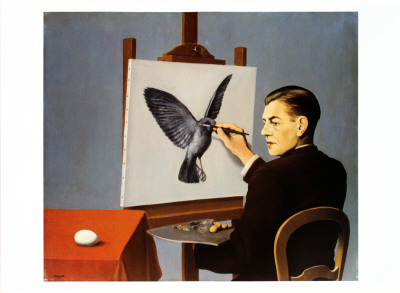
\includegraphics[width=0.7\textwidth]{img/egg-painter}
  \end{figure}
  \begin{center}
    \scriptsize
    \url{http://imagecache6.allposters.com/LRG/51/5141/9SSEG00Z.jpg}
  \end{center}
\end{frame}

\begin{frame}{Profesor $\rightarrow$ mentor}
  \begin{center}
    Cred în tine. (\textit{I believe in you})
  \end{center}
\end{frame}

\begin{frame}{O ,,modelare''}
  \begin{enumerate}
    \pause
    \item acoperișul casei: cunoștințe, informații
    \pause
    \item corpul casei: abilități, abordări, stil, rațiune
    \pause
    \item fundația casei: atitudine, mentalitate, valori, emoții
  \end{enumerate}
  \begin{itemize}
    \pause
    \item predarea/instruirea înseamnă adăugarea unor cărămizi
    \pause
    \item cele de mai jos sunt cele mai durabile (și rigide)
  \end{itemize}
\end{frame}

\begin{frame}{Lucrul la ,,fundație''}
  \begin{itemize}
    \pause
    \item \textit{care for you}, \textit{be there for you}
    \pause
    \item dezvăț (deconstrucție) pentru nivelurile de mai sus
    \pause
    \item \textit{growth mindset}
    \pause
    \item personalizare: pe profilul fiecăruia
    \pause
    \item emoțiile contează: ai în față un om, nu o mașină
  \end{itemize}
\end{frame}

\begin{frame}{Creativitatea}
  \begin{itemize}
    \pause
    \item nu se predă
    \pause
    \item poți consolida fundația pentru a înlesni creativitatea
    \pause
    \item deconstrucția să nu fie (prea) temută
  \end{itemize}
\end{frame}

\begin{frame}{Cum să predai de nota 10}
  \begin{itemize}
    \pause
    \item îți pasă, ai grijă
    \pause
    \item ești acolo
    \pause
    \item crezi în acea persoană (puternic și rar, pentru mentorat)
    \pause
    \item deconstruiești și construiești
    \pause
    \item suflet, nu doar minte și trup
  \end{itemize}
\end{frame}

\begin{frame}{În final}
  \pause
  \centering
  \LARGE{\textit{Am încredere în tine.}} \\
  \vspace{3mm}
  \hfill \normalsize{\textit{Răzvan Deaconescu}} \\
\end{frame}

\end{document}
